\begin{figure}
\centering
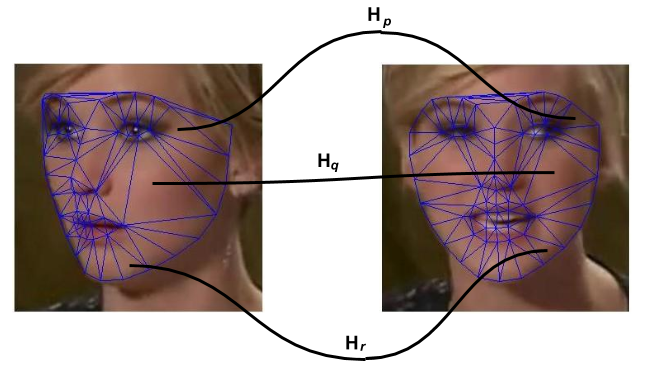
\includegraphics[width =11cm,height=6cm]{front/figures/triangulation.png}
\caption{Image shows the planes represented as triangles and correspondences between two views of
the same face. Note that each plane contains a fixed set of points irrespective of pose. For
example, one plane contains two ends of the eyebrows and the top of the nose.}
\label{fig:triangulation}
\end{figure}

Our face recognition pipeline is based on the framework of Write {\em et
al.}~\cite{Wright:2009:RFR:1495801.1496037} who claim that faces of a
particular individual lie in a low-dimensional subspace. 
%That is to say, if we have a set of faces
%of a particular person in varied conditions, it is possible to represent a new face of the same
%person using a linear combination of the rest of the faces. 
In their method, training samples are
represented as a 2D matrix, where each column represents a feature extracted from one training
image. The input test sample should then be represented as linear combination of samples from the
corresponding training samples of the same class (person). This problem has to be posed as an $l0$
minimization problem as it selects a combination of samples from training set. Based on recent advancement in sparse
representation and compressed sensing, the authors claim that when the solution is sparse enough, 
solving $l1$ minimization is equivalent to the $l0$ minimization problem. 
Using this insight, a solution can be obtained in polynomial time using linear programming models.
We use their implementation as the basis for our experiments, while we train using our dataset.
